\chapter{Theory}
\label{chap:theory}

This chapter provides an introduction to all relevant basis for this work. If you are already familiar with image processing and convolutional neural networks you can skip to \ref{sec:scattering_transform}. \\
The first Section \ref{sec:2D_image_processing} gives a general overview of image processing for readers unfamiliar with the concept. Then the Fourier transform is described in \ref{sec:fourier_transform} as an easier example of a filter that can be applied to images and changes the format of the their representation. In Section \ref{sec:scattering_transform} the Scattering Transform is introduced and its theoretical properties explained. It is followed by a general introduction to convolutional neural networks (CNNs) in Section \ref{sec:cnns} after which hybrid networks in the context of classification are described in Section \ref{section:hybrid_networks_for_classification}. Lastly, object detection is introduced in Section \ref{sec:object_detection} and the hybrid networks in the context of object detection conclude the chapter with Section \ref{sec:hybrid_networks_for_od}. 

\section{2D Image Processing}
\label{sec:2D_image_processing}

Image processing describes the application of different algorithms on images with the purpose of gaining certain information about it or changing its representation. Most of the time images are given as two dimensional pixel arrays where each entry denotes the intensity of that pixel. In the case of grayscale images the value is between 0 and 255 representing black and white respectively. When handling color images an additional 3rd dimension is added with three channels representing a red, green, blue (rgb) encoding. Each entry, again, has values between 0 and 255 representing color intensity. \\
Instead of imagining an image as a flat 2D object, it can also be seen as a terrain with surface, where the height of each coordinate is determined by the intensity of its value. An example of this is shown in Figure \ref{fig:image_surfaces}. 


\begin{figure}[!htb]
	\centering
	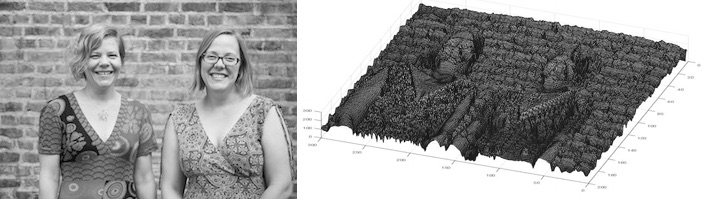
\includegraphics[width = 0.9\textwidth]{images/image_surfaces.jpg}
	\caption{Left: image represented as 2D flat surface. Right: image as 3D terrain with uneven surface. \protect\footnotemark}
	\label{fig:image_surfaces}
\end{figure}

\footnotetext{Figure taken from \url{https://plus.maths.org/content/fourier-transforms-images}}

%how does this work for color images?
%-> see scaling the scattering transform, just use 3 channels

Like every other surface, these images can now be approximated as the sum of many different two dimensional sine waves. 2D sine waves are defined as in Equation \ref{eq:2d_sine}, where $a$ is the amplitude and $h, k$ are the frequencies in $x$ and $y$ direction respectively.

\begin{equation}
	f = a \sin(h\cdot x+k\cdot y)
	\label{eq:2d_sine}
\end{equation}

To give an example of how this approximation looks like, Figure \ref{fig:2d_sine} shows examples of three different two dimensional sine waves. It can be observed that higher amplitudes dominate the resulting wave, i.e. determine the direction of the wave stronger than the smaller amplitudes. 


\begin{figure}[!htb]
	\centering
	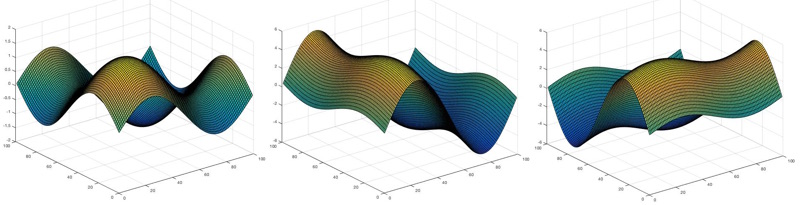
\includegraphics[width = \textwidth]{images/2d_sine.jpg}
	\caption{Left: $\sin(x) +\sin(y)$. Middle:  $5 \sin(x)+ \sin(y)$. Right: $	\sin(x)+5\sin(y)$. On the middle and right images the higher amplitudes of 5 dominate the resulting wave. \protect\footnotemark}
	\label{fig:2d_sine}
\end{figure}

\footnotetext{Figure taken from \url{https://plus.maths.org/content/fourier-transforms-images}}

\section{Fourier Transformation}
\label{sec:fourier_transform}

To get a better understanding of the Scattering Transform an explanation of a simpler and more commonly used transform is briefly discussed first in form of the Fourier Transform (FT). A FT decomposes a signal into the frequencies that make it up.

\subsection{One Dimensional FT} 

In the case of one dimensional signals, such as an audio signal, the decomposition are the coefficients of the sine waves representing the signal. A good example of this would be the decomposition of an audio signal. The FT is defined by Equation \ref{eq:forward_FT} for any real number $\omega$ and any integrable function $f:\mathbb{R} \rightarrow \mathbb{C}$. 

\begin{equation}
	\tilde{f}(\omega) = \int_{-\infty}^{\infty} f(x)\ e^{-2\pi i x \omega}dx
	\label{eq:forward_FT}
\end{equation} 

To get back to the Fourier domain when given a frequency, the inverse Fourier transform defined in Equation \ref{eq:inverse_FT} is used.  \\

\begin{equation}
	f(x) = \int_{-\infty}^{\infty} \tilde{f}(\omega)\ e^{2 \pi i x \omega}d\omega
	\label{eq:inverse_FT}
\end{equation}

When using discrete instead of continuous functions, the integrals in the definitions become sums. Then the definition of the forward FT is given in Equation \ref{eq:forward_FT_dis} and in Equation \ref{eq:inverse_FT_dis} for the inverse FT. 

\begin{equation}
\tilde{f}(\omega) = \sum_{x=1}^{n} f(x)\ e^{-2\pi i x \omega}
\label{eq:forward_FT_dis}
\end{equation} 

\begin{equation}
f(x) = \sum_{x=1}^{n} \tilde{f}(\omega)\ e^{2 \pi i x \omega}
\label{eq:inverse_FT_dis}
\end{equation}

\subsection{Two Dimensional FT}

Since images are two dimensional objects the Fourier transform needs to be extended. The Fourier transform then becomes a complex function of two or more real frequency variables $\omega_1, \omega_2$. Since images are finite objects the discrete version of the two dimensional Fourier transform is given in equation \ref{eq:forward_FT_2D} for the forward case and in equation \ref{eq:inverse_FT_2D} for the inverse case.

\begin{equation}
	\tilde{f}(\omega_1, \omega_2) = \sum_{x=1}^{n} \sum_{y=1}^{m} f(x,y)\ e^{-2\pi i (\omega_1 \cdot x + \omega_2 \cdot y)}
\label{eq:forward_FT_2D}
\end{equation}

\begin{equation}
f(x, y) = \sum_{x=1}^{n} \sum_{y=1}^{m} \tilde{f}(\omega_1, \omega_2)\ e^{2\pi i (\omega_1 \cdot x + \omega_2 \cdot y)}
\label{eq:inverse_FT_2D}
\end{equation}


\section{Scattering Transform}
\label{sec:scattering_transform}

This section explains the details of the Scattering Transform. It starts by explaining the basic functionality and adds functionality in every subsection. Subsection \ref{subsec:filter_bank} describes a combination of multiple wavelet filters called filter bank. Subsection \ref{subsec:scattering_path} shows how wavelets can be combined sequentially. The scattering networks described in Subsection \ref{subsec:scattering_networks} are a parallel and sequential combination of the wavelet filters that is also later used in the experiments. The section is concluded by a presentation and discussion of the properties of the Scattering Transform in Subsection \ref{subsec:properties}. \\
A transformation from the time to the frequency domain cannot only be performed by using the sine but in principal with any given periodic function.
Wavelets are wave-like oscillation with an amplitude that begin and end at zero. In most use cases wavelets are specifically crafted to have certain properties. 
The Scattering Transform is based on a Morlet wavelet, which is defined in equation \ref{eq:morlet2d}.

\begin{equation}
\psi(u) = C_1 (e^{iu.\xi} - C_2) e^{\frac{-|u|^2}{2\sigma^2}}
\label{eq:morlet2d}
\end{equation}


where $C_1$ and $C_2$ are constants. $C_2$ is chosen such that $\int \psi(u) du = 0$, $u.\xi$ denotes the inner product of $u$ and $\xi$, and $|u|^2$ is the norm in $\mathbb{R}^2$. 
Figure \ref{fig:morlet1d} shows the real and complex part of a Morlet wavelet.

\begin{figure}[!htb]
	\centering
	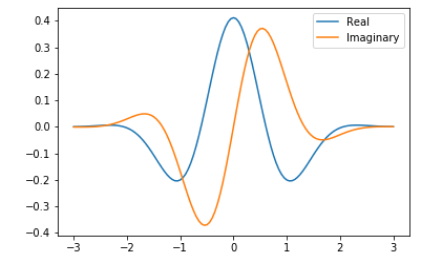
\includegraphics[width = 0.9\textwidth]{images/Morlet_wavelet_1D.png}
	\caption{Real and Complex part of Morlet wavelet in 1D. \protect\footnotemark}
	\label{fig:morlet1d}
\end{figure}

\footnotetext{Figure taken from \url{https://pdfs.semanticscholar.org/c354/c467d126e05f63c43b5ab2af9d0c652dfe3e.pdf}}

Similar to the Fourier transform the Morlet wavelet can also be extended to multiple dimensions. 
Figure \ref{fig:morlet2d} shows the 2 dimensional Morlet wavelet with parameters $\sigma = 0.85$ and $\xi = \frac{3\pi}{4}$. These parameters are taken from \cite{scatteringTransform2012}. No additional fine tuning w.r.t. to these parameters is done in this paper. 

\begin{figure}[!htb]
	\centering
	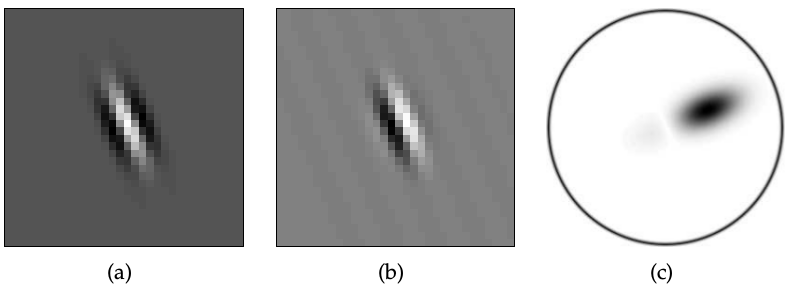
\includegraphics[width = 0.9\textwidth]{images/morlet2d.png}
	\caption{Complex morlet wavelet. a) Real part of $\psi$. b) Imaginary part of $\psi$. c) Fourier modulus $|\hat{\psi}|$. Image taken from \cite{scatteringTransform2012}.}
	\label{fig:morlet2d}
\end{figure}

\subsection{Filter Bank}
\label{subsec:filter_bank}

A wavelet transform filters $x$ using a family of wavelets: $\{x \star \psi_\lambda (u)\}_\lambda$. It is computed with a filter bank of dilated and rotated wavelets having no orthogonality property. The filter bank has four parameters: $M, N, J, L$ where $M,N$ stand for the initial spatial size of the input, $J$ is the scaling parameter and $L$ is the number of angles used for the wavelet transform. $J$ determines the size of the downsampling for the filters. The new output is downsampled by $2^{2\cdot J}$, i.e. An input image of size $(32, 32)$ is downsampled by $J=1$ to be of size $(16,16)$ or by $J=2$ to be of size $(8,8)$. It is important to note that the filter bank is just an accumulation of filters and is independent of the data. \\
A visualization of the filter bank used in this work can be found in figure \ref{fig:viz_filter_bank}. The filters are shown for $J=0,1,2$ and $L=8$ different angles. The red blurry dot in the bottom is the result of a Gabor filter which is a sinosoidal wave multiplied with a Gaussian function. The Gabor Filter is used as a low-pass filter. 


\begin{figure}[!htb]
	\centering
	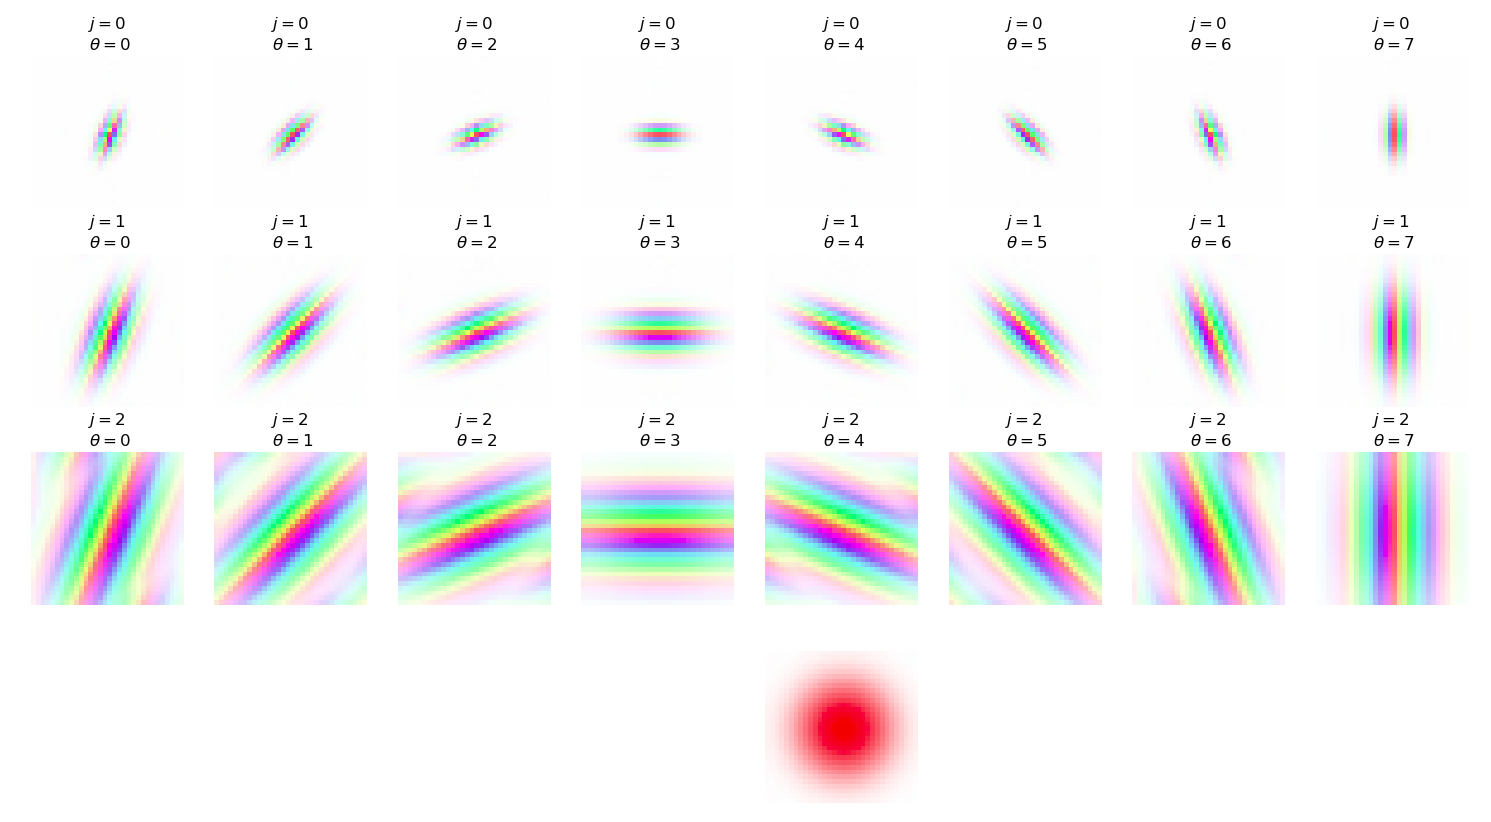
\includegraphics[width=\textwidth]{images/filter_bank_vis2.png}
	\caption{Visualization of the filter bank. The $j=0,1,2$ describe the different downsample sizes. The $\theta=0,...,7$ describe the different angles. For these images $N,M=32, L=8, J=3$. The contrast corresponds to the amplitude and the color to the phase. The blurry red dot in the bottom is the corresponding low-pass filter.}
	\label{fig:viz_filter_bank}
\end{figure}


\subsection{Scattering Paths}
\label{subsec:scattering_path}

To compute more and higher order scattering coefficients we iteratively apply the scattering transform. Let $U[\lambda]x = |x \star \psi_\lambda|$. A sequence $p = (\lambda_1, \lambda_2, ... \lambda_m)$ defines a \textit{path}, which is the ordered product: 
$$U[p]x = U[\lambda_m]...U[\lambda_2]U[\lambda_1] = | ||x \star \psi_{\lambda_1} | \star \psi_{\lambda_2}| ... | \star \psi_{\lambda_m}|. $$

A scattering transform along the path $p$ is defined as an integral, normalized by the response of a Dirac:

$$\bar{S}x(p) = \mu_p^{-1} \int U[p]x(u)du$$

with $\mu_p = \int U[p] \delta(u) du$. From this it follows that each scattering coefficient $\bar{S}x(p)$ is invariant to a translation of $x$. The scattering is Lipschitz continuous to deformations as opposed to the Fourier transform modulus.

%TODO what does that mean and what property does the Fourier transform modulus have?

\subsection{Scattering Networks}
\label{subsec:scattering_networks}


Scattering Networks are the result of all previously explained concepts. There are $m$ layers in the network, where every $m$ describes the length of the scattering paths in that layer. $m$ is also called order because it describes the number of consecutive scattering applications in that path. A scattering network is a tree that starts with a single root node in layer $m=0$ and branches out for every further layer with branching factor $L$. The scattering network is a collection of filters through which data can be forwarded as in any other computational graph. In contrast to most conventional CNN architectures (some use skip connections) the output is not only taken from the last layer, but from every single node in that network. An example of a scattering network with $L=4$ and $m=2$ is shown in figure \ref{fig:scattering_network}. The nodes describe the filters that are independent of the data, i.e. $U[\lambda_1]f$ for the first layer. The blue arrows indicate the outputs at every node, i.e. the scattering coefficients that result from applying this particular scattering path to data for example $S_J[\lambda_1]f$ for a node in the first layer. The root node $U_J[\theta]f = f \star \phi_J$ is the low-pass filter which is in this case a Gabor filter. \\
In \cite{scatteringTransform2012} it is shown that using more than $m=2$ produces a lot of unnecessary computation because most of the information from data is already captured in the second-order scattering coefficients. For practical purposes this paper from now on assumes that networks are at maximum $m=2$ layers deep and in this paper for some applications $m=1$ only. 
The total number of filters $k_1,k_2$ and therefore also the total number of outputs per datapoint are shown in Equation \ref{eq:order1_num_filters} for $m=1$ and in Equation \ref{eq:order2_num_filters} for $m=2$.
\begin{equation}
k_1 = i \cdot (1 + JL) 
\label{eq:order1_num_filters}
\end{equation} 
\begin{equation}
k_2 = i \cdot (1 + JL + \frac{1}{2}J(J-1)L^2)
\label{eq:order2_num_filters}
\end{equation}
$i$ denotes the number of input channels of the input data which is 3 for most applications since RGB images are used. In the case of RGB images the scattering transformation is applied for every channel separately. Figure \ref{fig:scattering_network} is only showing a network for one abstract $J$. Given that $J$ describes the factor by which the outputs are downsampled it also has to be factored in the Equations \ref{eq:order1_num_filters} and \ref{eq:order2_num_filters}. Lastly, it should be noted that the output of the scattering network all have the same downsampled size determined by $J$ even if the filters have different sizes. This is achieved by subsampling the current scattering coefficients in the Fourier domain such that the output size is the desired one. To make this more clear an example is provided: A scattering network with $N,M = 32; J=2; L=8$ is initialized. The network is applied on an RGB image. Therefore there are $3 \cdot (1+2 \cdot 8) = 51$ outputs of size $(8,8)$ because of the downsampling factor $J=2$. 
\begin{figure}[!htb]
	\centering
	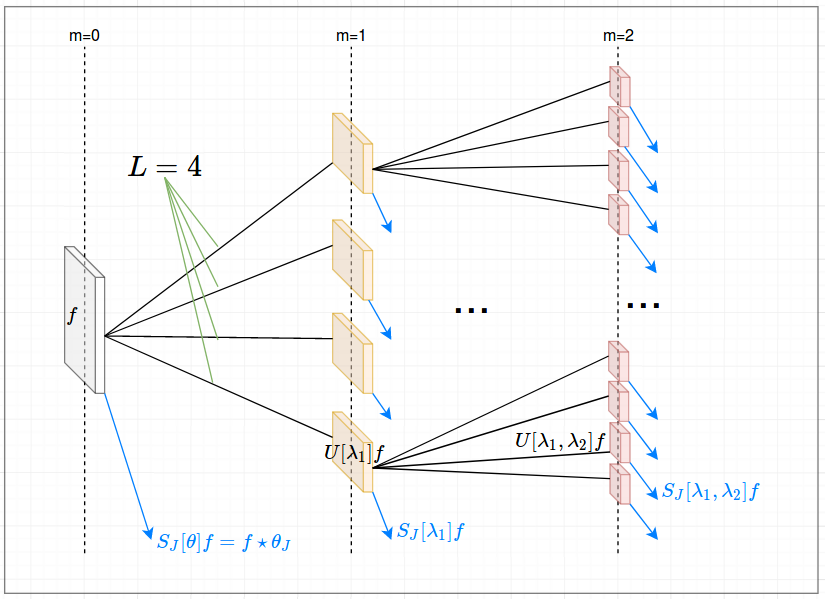
\includegraphics[width = 0.75\textwidth]{images/scattering_network_overview.png}
	\caption{Representation of a scattering network. Each filter is described by its path, e.g. $U[\lambda_1]f$. Every blue arrow describes an output at the particular filter. The $m=0,1,2$ describe the number of iterative applications of the scattering transform. $L=4$ is the branching factor in the network also known as the number of angles for the filter. The filters}
	\label{fig:scattering_network}
\end{figure}

The filters are applied in a convolutional manner, i.e. every point in the feature map is the result of the filter applied on a particular patch in the previous image or feature map. In comparison to the way convolution is described in section \ref{sec:cnns} the convolution is implemented through the Fourier Transform. By applying the inverse Fourier transform  ${\mathcal F}^{-1}$, we can write:

$$ f*g={\mathcal {F}}^{-1}{\big \{}{\mathcal {F}}\{f\}\cdot {\mathcal {F}}\{g\}{\big \}}$$

Instead of sliding a filter over the image, both the filter and the image are transformed in Fourier space and multiplied point-wise. The result of the point-wise multiplication is transformed back through the inverse Fourier Transform. The feature maps have a meaning that is understandable in human terms and can be analyzed visually. For two different images the 0th order, first order and second order scattering coefficients have been visualized in Figure \ref{fig:example1_coefficients} and \ref{fig:example_cat_coefficients}. Subfigure a) shows the original image. Subfigures b),c) and d) show the 0th to second order scattering coefficients respectively. The number of filters grows as described in Equation \ref{eq:order1_num_filters} and Equation \ref{eq:order2_num_filters}. Through this example it is very clear that the filters primarily encode geometric information, i.e. edges and corners of the object in the image. To get an  impression of the scattering coefficients in a more realistic setting, an additional image is analyzed in figure \ref{fig:example_cat_coefficients}. As one can see in the cat image, the scattering coefficients are also interpretable in terms of geometric properties of the cat. Additional examples are shown in the appendix. A comparison of the images in the appendix and in this section suggests that the scattering transform is equivariant w.r.t transformation. This means that the translation of an object in the image corresponds to a similar or at least proportional translation in the feature map. This is a desirable property for object detection and is also in aligment with the description of the following Subsection \ref{subsec:properties} when the distinction between local invariance and global equivariance is made. 

\fboxsep=0mm%padding thickness
\fboxrule=1pt%border thickness

\begin{figure}[!htb]
	\centering
	\begin{tabular}{cc}
		\subfloat[]{\fbox{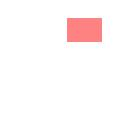
\includegraphics[width=4.5cm]{images/0000011_00.jpg}}} 
		& \subfloat[]{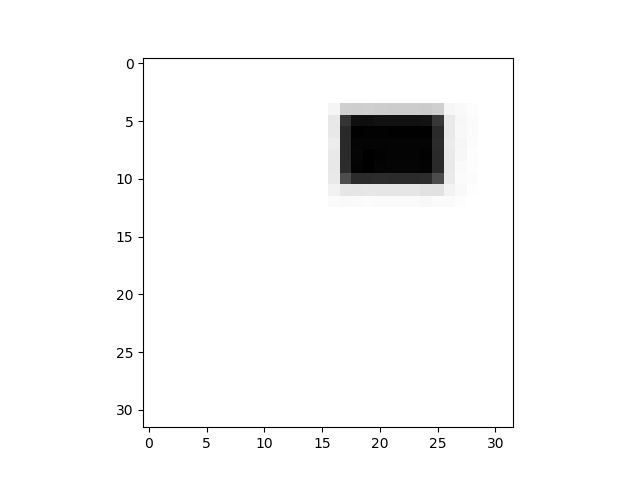
\includegraphics[width=7cm]{images/example1_0ord.png}}\\
		
		\subfloat[]{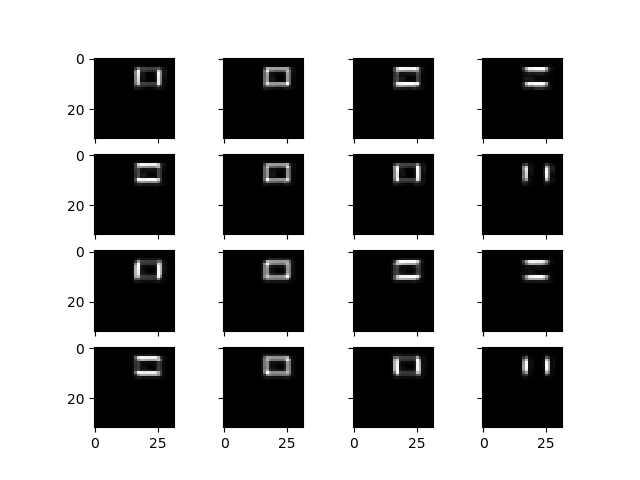
\includegraphics[width=7cm]{images/example1_1ord.png}} &
		\subfloat[]{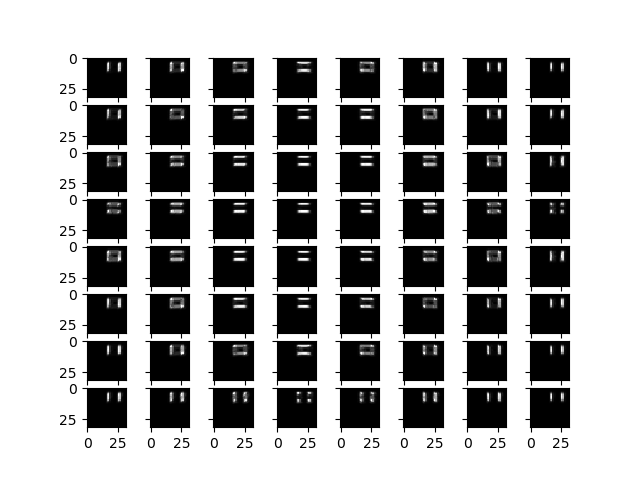
\includegraphics[width=8cm]{images/example1_2ord.png}}
	\end{tabular}
	\caption{Image taken from a toy dataset created for this work. a) Original image; b) 0th order scattering coefficients, i.e. a Gaussian low-pass filter; c) First order scattering coefficients; d) Second order scattering coefficients}
	\label{fig:example1_coefficients}
\end{figure}

\begin{figure}[!htb]
	\centering
	\begin{tabular}{cc}
		\subfloat[]{\fbox{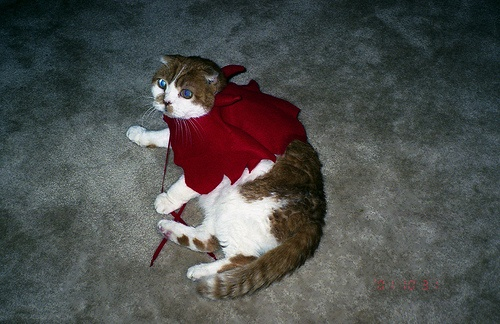
\includegraphics[width=4.5cm]{images/cat_example.jpg}}} 
		& \subfloat[]{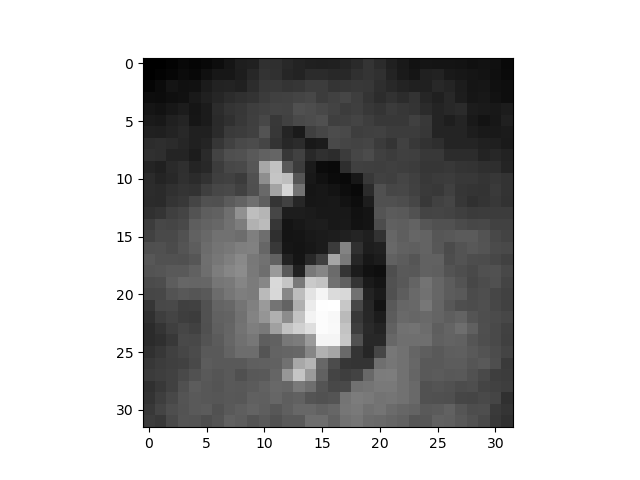
\includegraphics[width=7cm]{images/example_cat_0ord.png}}\\
		
		\subfloat[]{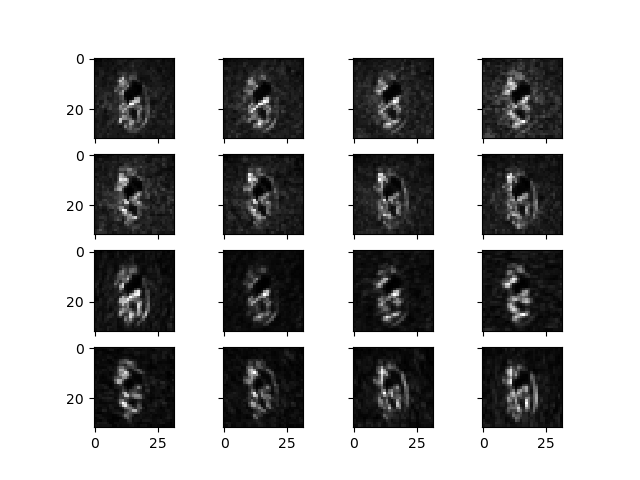
\includegraphics[width=7cm]{images/example_cat_1ord.png}} &
		\subfloat[]{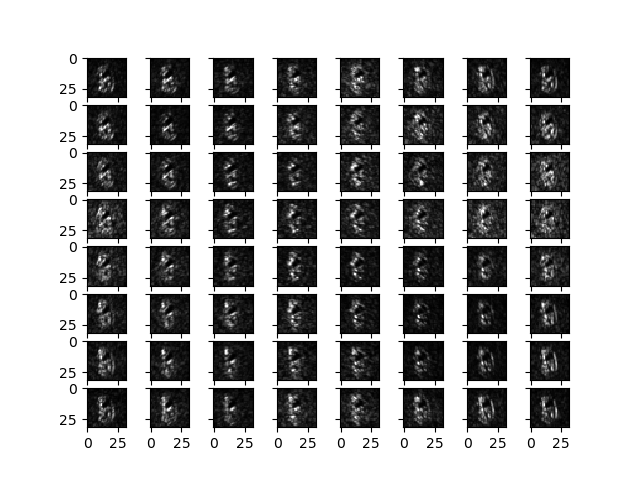
\includegraphics[width=8cm]{images/example_cat_2ord.png}}
	\end{tabular}
	\caption{Image taken from the VOC dataset. a) Original image; b) 0th order scattering coefficients, i.e. a Gaussian low-pass filter; c) First order scattering coefficients; d) Second order scattering coefficients}
	\label{fig:example_cat_coefficients}
\end{figure}

\subsection{Properties of the Scattering Transform}
\label{subsec:properties}

%TODO: How detailed? Just hint at it or copy entire section of original paper?
%-> rather detailed. everything should be clear

In this subsection the properties of the scattering transform as used in this work are layed out and the reasons for the properties are pointed out but not proven. For a more detailed explanation and references to proofs we refer the reader to the original paper \cite{scatteringTransform2012}. \\
A wavelet is a localized waveform and therefore stable to deformations. This is an upgrade to the sinusoidal waves of the Fourier transform which do not have this property. Before the properties can be explained the concepts of invariance and equivariance are defined. 
A function $f$ is invariant w.r.t to a transformation $T$ if the transformation does not change the outcome of the function when applied to the input $x$ as described in \ref{eq:invariance}.
\begin{equation}
f(Tx) = f(x)
\label{eq:invariance}
\end{equation}
A function $f$ is equivariant w.r.t to a transformation $T$ if the outcome of the function when applied to the input is transformed in a similar fashion as the input as shown in \ref{eq:equivariance}. Equivariance with respect to translation, for example, means the feature map of the filter reflects that translation in a proportional manner.
\begin{equation}
f(Tx) = Tf(x)
\label{eq:equivariance}
\end{equation}
A wavelet transform computes convolutions with wavelets. It is thus translation equivariant not invariant. To achieve local invariance a non-linearity must be added. The $\textbf{L}^1(\mathbb{R}^2)$ norm is chosen as the non-linearity. 
The invariance also only holds locally for displacements $c$ with $|c| << 2^J$. This means that during the reduction to smaller feature maps the scattering transform does not lose any information on the object but still keeps global equivariance. \\
Compared to the Fourier transform modulus, which is also invariant to deformations, the scattering transform is Lipschitz continuous to deformations, i.e. the change in the scattering coefficients is bounded and determined by the change in the deformed object. Deformation  stability of the Scattering Transform is  obtained  with  localized wavelet filters which separate the image variations at multiple scales and orientations. \\
L. Sifre and S. Mallat  \cite{RotationScalingDeformationSifre2013} show that the Scattering Transform also naturally fulfills global equivariance while having local invariance w.r.t. scale and rotation because of the Morlet wavelet.

\subsubsection{Discussion of the Properties}

In this work the scattering transform is applied to object detection. In previous works the scattering transform has mainly been applied to image classification. In the following a short distinction between the two tasks is presented. For image classification invariance w.r.t. rotation, translation, scale and deformation are all positive attributes because every image corresponds to exactly one category. In the context of object detection invariances can be problematic. If a transform is applied to an object the object detection algorithm should still be able to identify the object correctly thereby showing invariance but also produce a new and adapted bounding box thereby showing equivariance. Since the Scattering Transform shows local invariance and global equivariance the problems of invariance are not given as long as $J$ is sufficiently small, i.e. the image is not reduced too much. The empirical results, i.e. figures \ref{fig:example1_coefficients}, \ref{fig:example_cat_coefficients} and appendix suggest translation equivariance instead of invariance. Equivariance is a desirable property for object detection and therefore not problematic. Similar results are also seen for scale as shown in the appendix. \\
Given this theoretical insight this work proposes a specific kind of hybrid network which includes information from both a conventional CNN and the scattering networks which is described in Subsection \ref{subsec:parallel_hybrid}. 

     
 \section{Convolutional Neural Networks}
 \label{sec:cnns}
 
 For most image-related tasks, i.e. classification or object detection, a picture is used as a collection of pixels. However, not all pixels are equally important and subsets of the entire image form meaningfully connected subcollections. This might be a face in a photo of a family gathering. For humans the ability to detect these features and contextualize them comes naturally, for computers it does not. Therefore convolutional neural networks (CNNs) \cite{LeCun1989BackpropagationAT} are used. Convolutions are essentially just the application of filters on an image. The filter is applied at every possible location in the image, as described in figure \ref{fig:convolution}. In formulas the application of a filter through convolution will be denoted with the convolution operator $\star$.
 
 \begin{figure}[!htb]
    	\centering
    	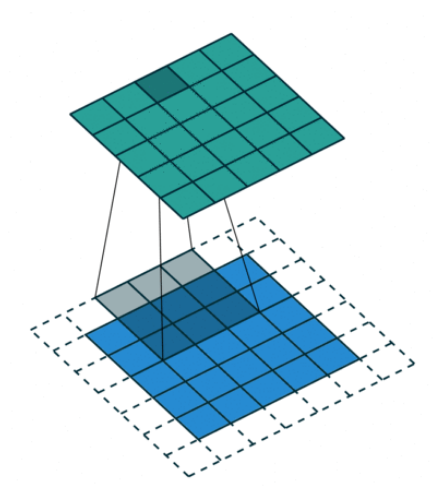
\includegraphics[width=0.5\textwidth]{images/convolution.png}
    	\caption{3x3 convolution on 5x5 image. Resulting image is also 5x5 due to the padding of size 1 added to the original image. \protect\footnotemark}
    	\label{fig:convolution}
 \end{figure}
 
 \footnotetext{Figure taken from and animated version at \url{https://towardsdatascience.com/types-of-convolutions-in-deep-learning-717013397f4d}}
 
 In CNNs there are multiple stages of filters in sequential order and multiple filters per layer. That means at every stage of the network different filters are applied on the outcome of an earlier step. The filters are assumed to learn different features of the images. The later the stage, the higher the level of complexity of the feature to be learned. That means, that an early filter might learn simple attributes such as edges or colors while a later filter might learn more complex features such as an eye or a nose and the very last filters even more complex semantic objects such as a face. The weights are trained by backpropagation using stochastic gradient descent. They determine what each individual filter does. This means that every filter that is a applied on a given layer learns its specific function such that overall the best accuracy can be achieved. 
 
 As just explained in conventional CNNs the filters are trained. However, there are some approaches that use static filters. Static filters essentially encode prior knowledge which is important for two key reasons. First, it lessens the dependency on big labeled datasets since the filters already contain some information and do not need to adapt. Second, specific theoretical guarantees can be made for some filters. A filter can be invariant or equivariant w.r.t. a specific transformation. Equivariance is a desirable property for object detection while invariance is undesirable. The bounding boxes for an image with one object and another image with the same but transformed object should not be similar but also translated accordingly.
 The Scattering Transform is one approach that ensures equivariance/invariance w.r.t. specific transformations as explained in Subsection \ref{sec:scattering_transform}. 

\section{Hybrid Networks for Classification}
\label{section:hybrid_networks_for_classification}

In \cite{ScalingTheScatteringTransform2017} E. Oyallon et al construct a hybrid of the Scattering Transform and classic classification architectures. They remove the first couple of layers of a ResNet \cite{ResNet15} architecture and substitute it with a scattering network such that the image is first transformed by the Scattering Transform and the ResNet is then trained on the scattering coefficients. Their results show two important insights. First, the accuracies on most classification tasks such as MNIST are as good as when just training a ResNet architecture. Second, when using less datapoints or images with distortions the hybrid network outperforms the standard architecture. This paper attempts to extend these results on object detection which is explained in the following section. 

\section{Object Detection}
\label{sec:object_detection}

Object detection is a task within image processing where objects on a given image are supposed to be detected. These objects can be anything from buildings over cars to humans. The images are already annotated for training, i.e. a rectangle (or other representation) that approximates the object best is already placed over the picture with the associated class attached. An example of such an annotated image can be found in figure \ref*{fig:annot_example}.

\begin{figure}[!htb]
	\centering
	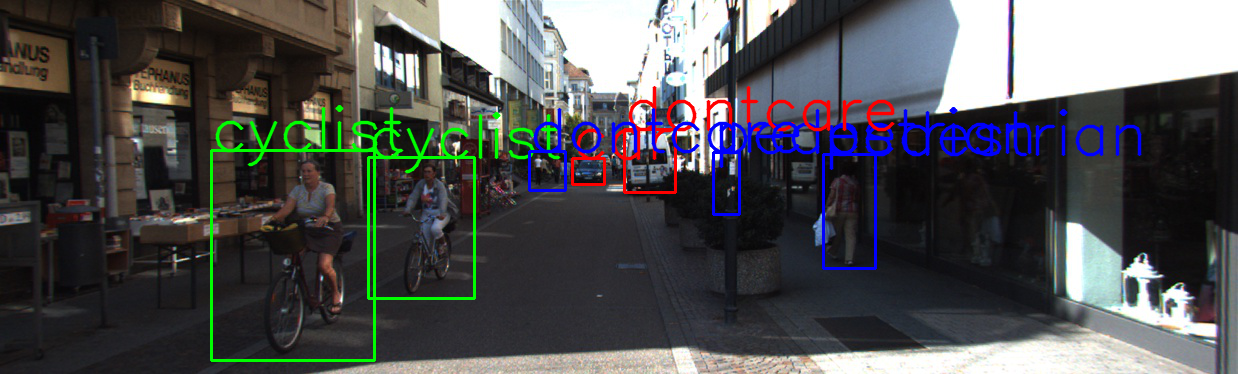
\includegraphics[width=0.9\textwidth]{images/Annotations_example.png}
	\caption{An example of a annotated image taken from the Kitti dataset. There are seven objects of four classes visible: cyclist, car, pedestrian and dontcare.}
	\label{fig:annot_example}
\end{figure}

Many methods have been explored to increase the accuracy of object detection ranging from sliding window approaches over hand crafted feature extraction to artificial neural networks. All current state of the art results for object detection are achieved by using Convolutional Neural Networks (CNN) in different ways. Broadly speaking object detection networks can be distinguished in one-stage and two-stage detectors. One-stage detectors are fully convolutional networks, e.g. YOLO \cite{yolo} or SSD \cite{SSD}. Two stage object detection networks have a region proposal method as their first part. This method can either be selective search as in the case of RCNN \cite{RCNN} or a region proposal network as in FastRCNN \cite{FastRCNN} or FasterRCNN \cite{FasterRCNN}. The second stage then consists of classifying the objects in the proposed regions and finding the most fitting bounding boxes. In this stage all previously named network types use a CNN for the classification. Therefore this work also uses a CNN as the backbone of the object detection. The object detection network that is used for this paper is discussed in the following subsection.

\subsection{Single Shot Multibox Detector (SSD)}

%How does it work?
The Single Shot Detector (SSD) is a fully convolutional object detection network \cite{SSD}. The SSD consists of two main components: an adapted version of a standard CNN used in classification tasks, i.e. VGG or ResNet, and extra feature layers that transform the features from the first part to meaningful information w.r.t. the final classes and their location. The final detections are then pushed through a Non-Maximum Suppression (NMS) operation to put a higher weight on probably correct detections and a lower weight on probably incorrect detections. Additionally NMS also merges all detections belonging to the same class and only keeps the bounding boxes with highest confidence for a given region thereby removing redundant encodings of the same object. 
A detailed graphical description of the SSD and VGG16 can be found in figure \ref{fig:SSD}. In the upper picture an overview of the SSD architecture can be seen. The data is piped through the adapted classification architecture, in this case VGG16. However, instead of connecting the output with a fully connected layer to the output layer it is now piped through the extra feature layers. Those are responsible for anchor boxes on the image with different feature sizes and aspect ratios. Anchor boxes are predefined boxes offered to the network such that it only has to choose the best fitting one instead of suggesting its own box proposals. The concept of anchor boxes and feature maps is visualized in Figure \ref{fig:SSD_feature_maps}.

\begin{figure}[!htb]
	\centering
	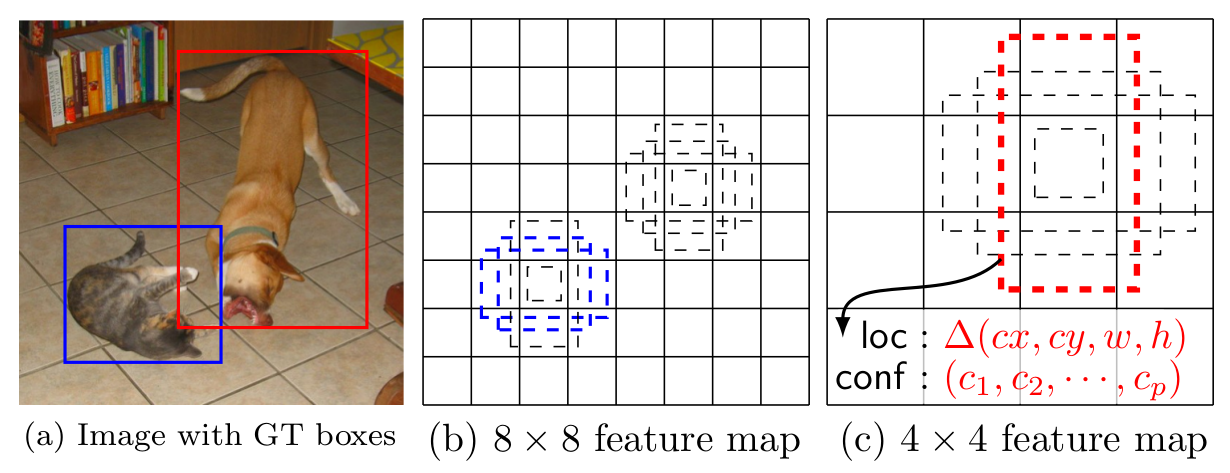
\includegraphics[width=\textwidth]{images/SSD_feature_maps}
	\caption{A graphical explanation of the feature maps and anchor boxes. The grid shows the feature map. The boxes with dotted contours describe different possible anchor boxes for one entry on the grid. Image from the original SSD paper \cite{SSD}.}
	\label{fig:SSD_feature_maps}
\end{figure}

Some of the combinations of feature sizes and aspect ratios will match an object on the image. The probability that an anchor box represents an object is evaluated by the confidence layers. There are a total of 8732 detections per image and class as a consequence of all convolutions described in Figure \ref{fig:SSD}. All detections that are bigger than a certain threshold are the output of the network. The VGG is just represented as a big box in the first image but a more detailed view is represented in the second. The main idea behind the VGG is to pipe the data through multiple convolutional layers that have decreasing feature map size but increasing number of channels. As already described in \ref{sec:cnns} the representations are increasingly large with increasing layer number. The reduction of the feature map size is done by a 2x2 max pooling operation which is a method to reduce the size of representations while keeping the most important information. For a theoretical introduction to max pooling or a general overview of CNNs see Schmidhubers overview paper \cite{SchmidhuberOverview}. 

\begin{figure}[!htb]
	\centering
	\begin{tabular}{c}
		\subfloat[]{\fbox{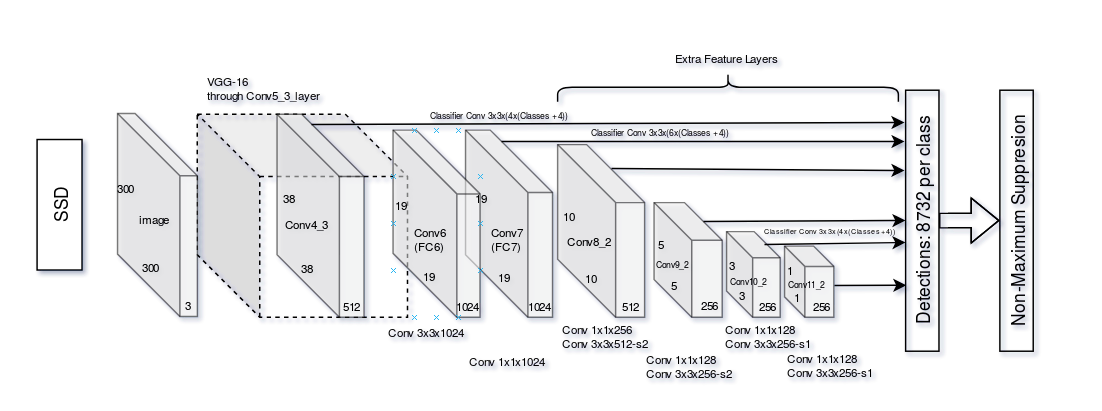
\includegraphics[width=\textwidth]{images/simple_ssd.png}}} 
		\\ \subfloat[]{\fbox{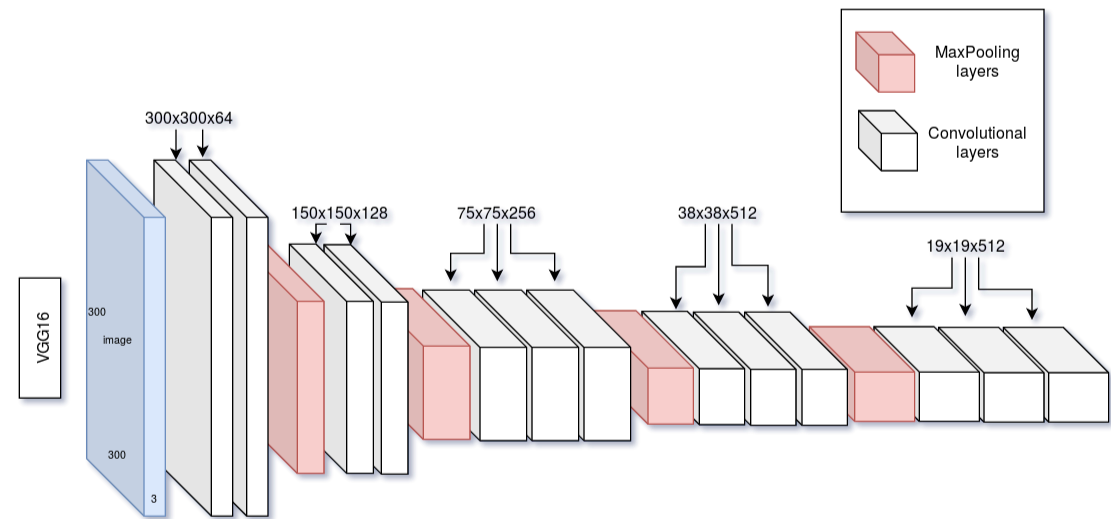
\includegraphics[width=\textwidth]{images/VGG16.png}}} 
	\end{tabular}
	\caption{Figure of the SSD network. a) Entire SSD with focus on extra feature layers and Non-Maximum Suppression. b) VGG16 in more detail. Explanations for the figures are in the respective section. The tensors NxNxC stand for the feature map size and number of channels, i.e. conv\_2\_1 has a feature map of 150x150 with 128 parallel channels. The red boxes describe $2x2$ max-pooling operations.}
	\label{fig:SSD}
\end{figure}

%why SSD instead of fast RCNN or faster RCNN
In its original paper \cite{SSD} the SSD performed very well on the PASCAL VOC2007 benchmark set, however, on most other object detection tasks, i.e. Kitti \cite{Geiger2013IJRR}, it is outperformed by fast R-CNN \cite{FastRCNN} or faster R-CNN \cite{FasterRCNN} two other architectures for object detection. In this work SSD is used instead of other architectures because it is comparably simple and easier to set up. Given that the task of this work is only to test whether the scattering transform can be used effectively to perform object detection, relative measures to the standard architecture are sufficient. However, there is no principal reason not to combine the scattering transform in the same way it is done in this paper with other object detection architectures if those are using convolutional layers (which is the current state of the art). This might be a suggestion for future work but is not part of this paper.


\section{Hybrid Networks for Object Detection}
\label{sec:hybrid_networks_for_od}

Hybrid networks in the context of this paper describe a combination of conventional object detection network architectures and the scattering transform. Note that this is similar to the hybrid networks as originally proposed by \cite{ScalingTheScatteringTransform2017} but extended to object detection. Two possible ways to combine the two techniques are described in the following. Subsection \ref{subsec:sequential_hybrid} describes the extension of the hybrid networks to object detection. Subsection \ref{subsec:parallel_hybrid} shows a new technique combining the two methods in a different way. 

\subsection{Sequential Hybrid Networks}
\label{subsec:sequential_hybrid}

Sequential hybrid networks describe an architecture in which the first couple of filters in a conventional object detection network have been replaced by the scattering transform. A general overview of the sequential architecture can be found in figure \ref{fig:sequential_scattering_overview}. The details of the implementation are found in figure \ref{fig:sequential_scattering_SSD} in the following chapter. 

\begin{figure}[!htb]
	\centering
	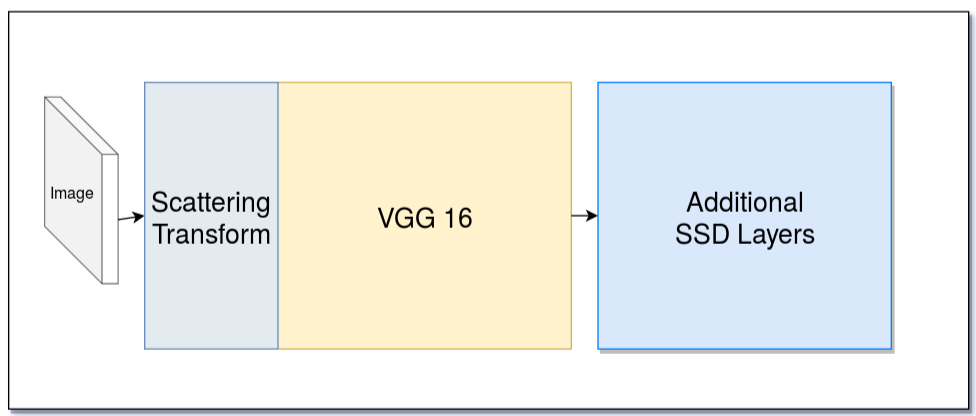
\includegraphics[width=\textwidth]{images/sequential_scattering_overview.png}
	\caption{General overview of the sequential scattering architecture.}
	\label{fig:sequential_scattering_overview}	
\end{figure}


\subsection{Parallel Hybrid Networks}
\label{subsec:parallel_hybrid}

Another possibility to combine the two networks is through concatenation during the forward pipeline. The intention here is to combine the strength of both techniques: the flexibility of the CNN with the robustness of the scattering transform. A general overview of the parallel architecture can be found in figure \ref{fig:parallel_scattering_overview} The details of the implementation are found in figure \ref{fig:parallel_scattering_SSD} in the following chapter. 

\begin{figure}[!htb]
	\centering
	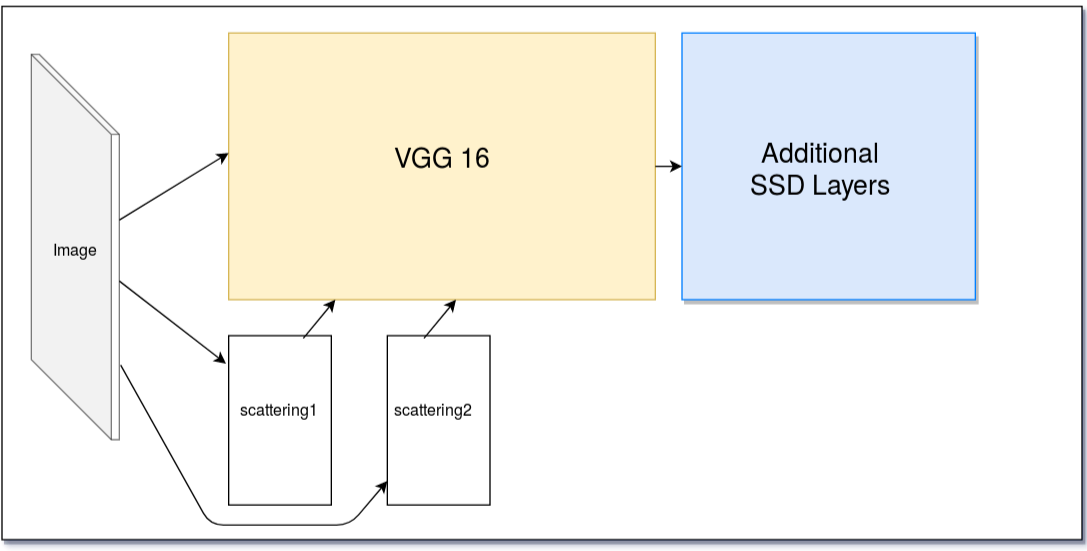
\includegraphics[width=\textwidth]{images/parallel_scattering_overview.png}
	\caption{General overview of the parallel scattering architecture.}
	\label{fig:parallel_scattering_overview}	
\end{figure}
